\bookchapter{Object Detection and YOLO}\label{ch:ai4}

\section*{Explanation}
A classifier says ``there is a ball in this picture''. A robot needs more: \emph{where} is the ball, how many robots are there, which one is a team mate? This task is \textbf{object detection}: for every object in the image the network outputs a \textbf{bounding box} (a rectangle around the object), a \textbf{class} and a \textbf{confidence}. Detection is the first step of every soccer robot's vision: from the box follow the distance and direction of the ball (Chapter~\ref{ch:ros4}). The best known family of fast detectors is called \textbf{YOLO} (``You Only Look Once''), because it finds all objects in one pass of one network. Understanding the pieces (boxes, IoU, grid, non-maximum suppression, mAP) is more valuable than knowing the latest version of the software, since all detectors use them.

\section*{Boxes and how to write them}
A box can be written in several ways, and mixing them up is a classic bug:
\begin{center}
\renewcommand{\arraystretch}{1.25}
\begin{tabular}{p{2.6cm}p{5.2cm}p{4.6cm}}
\textbf{Format} & \textbf{Numbers} & \textbf{Used by}\\ \hline
xyxy (corners) & $(x_1,y_1,x_2,y_2)$ in pixels & OpenCV drawing, many metrics\\
xywh (corner + size) & $(x_1,y_1,w,h)$ in pixels & COCO data set files\\
cxcywh normalised & $(c_x/W,\;c_y/H,\;w/W,\;h/H)$, all in $0..1$ & YOLO label files\\
\end{tabular}
\end{center}
\begin{example}
\textbf{A label file.} A ball with its centre at pixel $(400,300)$ and a size of $24\times24$ pixels in an image of $640\times480$ is stored in the YOLO text format as \texttt{0 0.625 0.625 0.0375 0.05}: class number $0$, $400/640=0.625$, $300/480=0.625$, $24/640=0.0375$, $24/480=0.05$. One line per object, one file per image, with the same name as the image. Normalised numbers stay valid when the image is resized.
\end{example}

\section*{IoU: how well do two boxes overlap?}
To compare a predicted box with the true box one uses the \textbf{intersection over union}:
\[
\mathrm{IoU}=\frac{\text{area of the overlap}}{\text{area of the union}}=\frac{|A\cap B|}{|A|+|B|-|A\cap B|}.
\]
It is $1$ for identical boxes, $0$ for boxes that do not touch. Typical rules: a detection is ``correct'' if its IoU with a true box is at least $0.5$.
\begin{center}
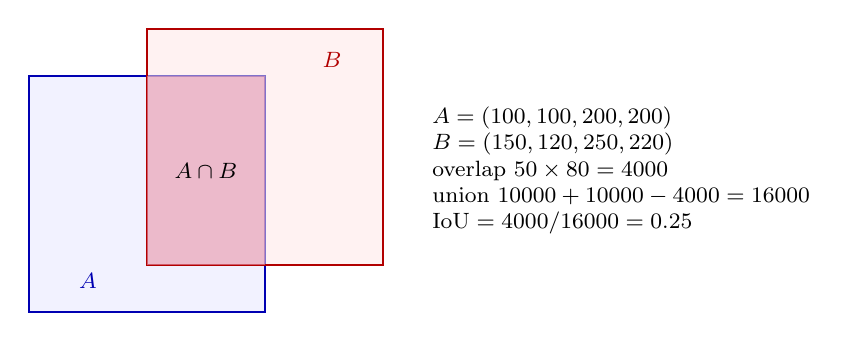
\begin{tikzpicture}
 \draw[thick,blue!70!black,fill=blue!10,fill opacity=0.5] (0,0) rectangle (3,3);
 \draw[thick,red!70!black,fill=red!10,fill opacity=0.5] (1.5,0.6) rectangle (4.5,3.6);
 \fill[purple!40,opacity=0.6] (1.5,0.6) rectangle (3,3);
 \node[font=\footnotesize,blue!70!black] at (0.75,0.4) {$A$};
 \node[font=\footnotesize,red!70!black] at (3.85,3.2) {$B$};
 \node[font=\footnotesize] at (2.25,1.8) {$A\cap B$};
 \node[font=\footnotesize,align=left,anchor=west] at (5.0,1.8) {$A=(100,100,200,200)$\\ $B=(150,120,250,220)$\\ overlap $50\times80=4000$\\ union $10000+10000-4000=16000$\\ $\mathrm{IoU}=4000/16000=0.25$};
\end{tikzpicture}
\captionof{figure}{The intersection over union of two boxes (numbers from the example; the figure is not to scale).}
\end{center}
\begin{verbatim}
def iou(a, b):                       # boxes as (x1, y1, x2, y2)
    x1, y1 = max(a[0], b[0]), max(a[1], b[1])
    x2, y2 = min(a[2], b[2]), min(a[3], b[3])
    inter = max(0, x2 - x1) * max(0, y2 - y1)
    area = lambda r: (r[2] - r[0]) * (r[3] - r[1])
    return inter / (area(a) + area(b) - inter)
\end{verbatim}
The code gives $0.25$ for the boxes of the figure. IoU is also used inside the training loss: a box loss based on IoU (variants called GIoU, DIoU, CIoU) tells the network not only whether the box is wrong but how.

\section*{The YOLO idea: a grid of predictions}
The image is covered by a grid. Every cell is responsible for objects whose centre lies in it and predicts: the offset of the box centre in the cell, the width and height, and a score for each class. The network is fully convolutional (Chapter~\ref{ch:ai3}), so ``the grid'' is just the spatial size of the last feature map: every position of the feature map gives one prediction. To find objects of very different sizes the detector uses \textbf{several feature maps with different strides}: stride $8$ (fine grid, for small objects such as a ball far away), $16$ and $32$ (coarse grid, for large objects such as a robot nearby). The part of the network that produces them is the \textbf{backbone} (a CNN as in Chapter~\ref{ch:ai3}) together with the \textbf{neck} (which mixes the feature maps of different scales), and the \textbf{head} computes boxes and classes.
\begin{center}
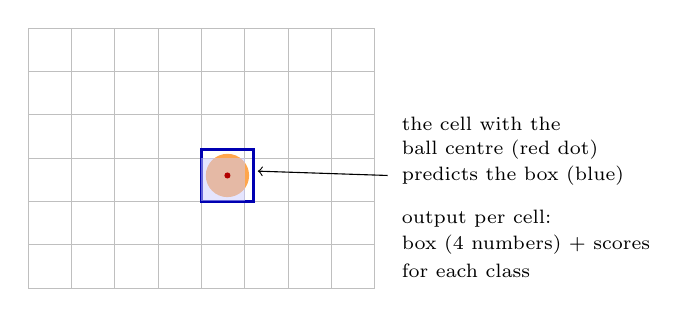
\begin{tikzpicture}[scale=0.55]
 \foreach \x in {0,...,8} \draw[gray!50] (\x,0)--(\x,6);
 \foreach \y in {0,...,6} \draw[gray!50] (0,\y)--(8,\y);
 \fill[orange!70] (4.6,2.6) circle (0.5);
 \draw[thick,blue!70!black] (4.0,2.0) rectangle (5.2,3.2);
 \fill[blue!20,opacity=0.5] (4,2) rectangle (5,3);
 \fill[red!70!black] (4.6,2.6) circle (2pt);
 \node[font=\scriptsize,anchor=west] at (8.4,3.8) {the cell with the};
 \node[font=\scriptsize,anchor=west] at (8.4,3.2) {ball centre (red dot)};
 \node[font=\scriptsize,anchor=west] at (8.4,2.6) {predicts the box (blue)};
 \draw[->] (8.3,2.6) -- (5.3,2.7);
 \node[font=\scriptsize,anchor=west] at (8.4,1.6) {output per cell:};
 \node[font=\scriptsize,anchor=west] at (8.4,1.0) {box (4 numbers) + scores};
 \node[font=\scriptsize,anchor=west] at (8.4,0.4) {for each class};
\end{tikzpicture}
\captionof{figure}{The grid idea (only one scale shown).}
\end{center}
\begin{example}
\textbf{How many predictions?} For an input of $640\times640$ and the strides $8,16,32$, the maps have $80\times80$, $40\times40$ and $20\times20$ cells: $6400+1600+400=8400$ predictions. With three classes (ball, robot, goal post), and in the common form that predicts $4$ box numbers plus one score per class, the output has the shape $(4+3)\times8400$. For a smaller input of $416\times416$: $52^2+26^2+13^2=3549$. Almost all of these predictions are ``nothing'' (the background). The network is trained to give them a low score.
\end{example}
Decoding one prediction is simple: for the cell in column $g_x=30$ and row $g_y=12$ of the stride-$16$ map, the cell centre is at $((30+0.5)\cdot16,\,(12+0.5)\cdot16)=(488,200)$ pixels, and the network adds a small learned offset and a size.

\section*{Non-maximum suppression}
A ball covers several cells, and neighbouring predictions all say ``ball'' with slightly different boxes. \textbf{Non-maximum suppression} (NMS) removes the duplicates: (1) sort all boxes of a class by score; (2) keep the best; (3) delete every other box whose IoU with the kept one is above a threshold (e.g.\ $0.5$); (4) repeat with the best of the rest.
\begin{verbatim}
def nms(boxes, scores, thr=0.5):
    order = np.argsort(scores)[::-1]
    keep = []
    while len(order):
        i = order[0]
        keep.append(int(i))
        order = np.array([j for j in order[1:]
                          if iou(boxes[i], boxes[j]) < thr])
    return keep
\end{verbatim}
\begin{example}
Four boxes with the scores $0.9,0.8,0.7,0.6$: $b_1=(100,100,200,200)$, $b_2=(110,105,205,210)$, $b_3=(300,150,360,210)$, $b_4=(105,95,195,195)$. The IoUs of $b_1$ with all four are $1.0,\,0.748,\,0.0,\,0.818$. NMS keeps $b_1$, removes $b_2$ and $b_4$ (IoU $>0.5$ with $b_1$), keeps $b_3$ (no overlap): result $[b_1,b_3]$. A threshold that is too low removes real neighbouring objects (two balls close together, a robot behind a robot); too high leaves duplicates. NMS is the slow, non-neural part of a detector, and its cost grows with the number of candidate boxes (Chapter~\ref{ch:ai9}).
\end{example}

\section*{Training a detector: the loss}
Training needs images with labelled boxes. For each true object the training procedure \textbf{assigns} a few predictions that are close to it, and the loss has two parts: a \textbf{box loss} (IoU-based, for the position and size) and a \textbf{class loss} (cross-entropy-like, Chapter~\ref{ch:prob}) for these predictions, while all other predictions are trained to say ``background''. Because only a handful of the $8400$ predictions are positive, the training must balance this heavy imbalance, which is solved inside the framework. You will rarely write these parts yourself, but you will tune three things: the data (Chapter~\ref{ch:ai5}), the input size and the model size.

\section*{Measuring quality: precision, recall, AP, mAP}
At a given score threshold a detection is a \textbf{true positive} (TP) if it has $\mathrm{IoU}\ge0.5$ with a not yet matched true box of the same class, otherwise a \textbf{false positive} (FP); true objects that nobody found are \textbf{false negatives} (FN).
\begin{align*}
\text{precision}&=\frac{TP}{TP+FP}\quad(\text{how many of my detections are right}),\\
\text{recall}&=\frac{TP}{TP+FN}\quad(\text{how many of the true objects I found}).
\end{align*}
Lowering the threshold gives more recall and less precision. The \textbf{average precision} (AP) is the area under the precision-recall curve for one class, and the \textbf{mAP} (mean AP) is the mean over the classes; \textbf{mAP@0.5} uses the IoU threshold $0.5$, \textbf{mAP@0.5:0.95} averages over the thresholds $0.5,0.55,\dots,0.95$ and rewards precise boxes.
\begin{example}
\textbf{Computing an AP.} A detector delivers $8$ detections of the class ball, sorted by score, there are $5$ true balls. Correct (1) or wrong (0): $1,1,0,1,0,1,0,0$. After each detection, recall $=TP/5$ and precision $=TP/(\text{number of detections so far})$:
\begin{center}
\renewcommand{\arraystretch}{1.15}
\begin{tabular}{r|cccccccc}
detection & 1&2&3&4&5&6&7&8\\ \hline
recall & 0.2&0.4&0.4&0.6&0.6&0.8&0.8&0.8\\
precision & 1.00&1.00&0.67&0.75&0.60&0.67&0.57&0.50\\
\end{tabular}
\end{center}
One makes the precision curve monotone (each value is replaced by the maximum to its right) and sums the areas of the steps: $0.2\cdot1.00+0.2\cdot1.00+0.2\cdot0.75+0.2\cdot0.667=\mathbf{0.683}$ (the fifth ball is never found, so recall stops at $0.8$). Code for this is in the answers of the problems; it gives $0.6833$.
\end{example}
For a robot the mAP is not the whole truth. What counts is the performance \emph{at the distances and in the light of the field}: a ball in the left corner at $10$\,m matters, a ball at $0.5$\,m in the foreground is easy. Evaluate separately per size and per distance (Chapter~\ref{ch:ai5}), and also check what the false positives are (a white shoe, a spot on the carpet).

\section*{Small objects}
The pixel size of the ball follows from the pinhole model of Chapter~\ref{ch:hw4}: $d_\text{px}=f_\text{px}D/Z$. With $f_\text{px}=554$ (a $640$-pixel-wide image, field of view about $60^\circ$) and $D=0.13$\,m:
\begin{center}
\renewcommand{\arraystretch}{1.15}
\begin{tabular}{r|ccccc}
distance $Z$ (m) & 1 & 3 & 6 & 10 & 15\\ \hline
ball diameter (px) & 72 & 24 & 12 & 7.2 & 4.8\\
\end{tabular}
\end{center}
A ball at $10$\,m is only $7$ pixels wide, smaller than one cell of the finest grid (stride $8$). If you shrink the camera image from $640$ to $320$ pixels to save time, the ball at $10$\,m has $3.6$ pixels and is practically invisible. This simple computation decides how far the detector can see; it is better than guessing. Remedies: higher input resolution (slower), a camera with a narrower field of view or a higher resolution, \textbf{tiling} (cut the image into overlapping crops), or a cheaper pre-detector that proposes where to look (for example a colour filter with a window around the candidates, as in Chapter~\ref{ch:ros6}, followed by the network on the small crop).

\section*{Using a ready-made detector}
In practice you start from a \textbf{pre-trained} model and \textbf{fine-tune} it on your own images. The most used tool of the YOLO family is the Python package \texttt{ultralytics}; its use is short (the code was not run when this book was written; versions and file names change quickly, so follow the documentation of the current release):
\begin{verbatim}
from ultralytics import YOLO
model = YOLO("yolov8n.pt")                 # small pre-trained model
model.train(data="soccer.yaml", epochs=100, imgsz=640)
results = model("frame.jpg")               # inference
for box in results[0].boxes:
    print(box.cls, box.conf, box.xyxy)
\end{verbatim}
\texttt{soccer.yaml} lists the folders of the images and the names of the classes. \textbf{Check the licence}: some popular implementations are released under the AGPL, which has strong conditions when you distribute software or offer it as a network service; other detectors are available under more permissive licences. For a school project this is usually no problem, for a company product it is; the same is true for the licence of the \emph{pre-trained weights} and of the data.

\subsection*{More than boxes}
The same networks can output more: \textbf{segmentation masks} (the exact pixels of the field lines or of the ball), \textbf{keypoints} (the joints of a robot or a human, the corners of the penalty area for self-localisation) and \textbf{oriented boxes}. A detector is run on every frame; to follow an object over time and to give it a stable identity one adds a \textbf{tracker} (a Kalman filter on the position of the boxes, Part~\ref{part:control}), which also fills the gaps when the detector misses one frame.

\begin{aibox}[From the detector to the robot's decision]
The chain is: camera image $\rightarrow$ network $\rightarrow$ boxes $\rightarrow$ NMS $\rightarrow$ ball pixel and size $\rightarrow$ distance and direction (Chapter~\ref{ch:ros4}) $\rightarrow$ position on the field $\rightarrow$ behaviour. Every error is amplified along the way: an error of $2$ pixels in the box width at $6$\,m ($12$ pixels) is $17\,\%$ in the distance. Therefore look at the size of the box, not only whether it exists, and filter the result over time.
\end{aibox}

\section*{Practice problems}
\begin{enumerate}[label=\textbf{\thechapter.\arabic*}]
  \item Compute the IoU of $A=(0,0,100,100)$ and $B=(50,50,150,150)$ and of $A$ and $C=(100,0,200,100)$.
  \item Convert the pixel box $(x_1,y_1,x_2,y_2)=(300,200,360,260)$ in an image of $640\times480$ to the YOLO label format (class $2$).
  \item An input of $512\times512$ with strides $8,16,32$: how many predictions? Which fraction of them lies on the finest grid?
  \item Three boxes of the same class: $(10,10,110,110)$ with $0.95$, $(20,20,120,120)$ with $0.90$ and $(200,200,260,260)$ with $0.80$. Run NMS by hand with the threshold $0.5$.
  \item Why must NMS be applied \emph{per class}? What can go wrong if it is applied to all classes together (think of a ball in front of a robot's foot)?
  \item A detector gives these detections of the class robot, sorted by score: $1,0,1,1,0,1$ (correct=1), and there are $5$ true robots. Compute the precision and recall after each detection and the AP.
  \item The ball has $D=0.13$\,m. With $f_\text{px}=700$ (an image $800$ pixels wide), at which distance is the ball $8$ pixels wide (one cell at stride $8$)? Repeat for an image that was reduced to half the size.
  \item A detector has high mAP@0.5 but low mAP@0.5:0.95. What does it tell you about its boxes? Would this be a problem for estimating distance from the box width?
  \item The ball's box in the image has a width of $18$ pixels, and the true width of the ball is $0.13$\,m ($f_\text{px}=554$). Compute the distance, and the distance if the box is $2$ pixels too wide. What is the relative error?
  \item[\textbf{\thechapter.10}$\star$] Implement \texttt{average\_precision(flags, n\_gt)} that follows the example of the chapter, and the function \texttt{match(dets, gts, thr)} that takes detections (box, score) and true boxes of one image and returns the list of TP/FP flags sorted by score (each true box may be matched only once). Test it with two true boxes and three detections of your choice.
\end{enumerate}
